% !TeX spellcheck = cs_CZ
%{\tikzset{external/prefix={tikz/MAI/}}
% \tikzset{external/figure name/.add={ch11_}{}}
%---------------------------------------------------------------------------------------------------
% file NM.tex
%---------------------------------------------------------------------------------------------------
\chapter{Numerické metody}
\minitoc

  \section{Úvodní slovo}
    Numerické metody jsou metody, které na rozdíl od metod analytických poskytujících spojité řešení
    na určité předem definované oblasti, dávají čísel\-né řešení v předem zvolených diskrétních
    bodech této oblasti. Na rozdíl od analytických metod toto řešení většinou nebývá přesné, ale
    představuje pouze jeho aproximaci, která je zatížena určitou chybou.
    
    Možnosti analytických metod se již asi třicet let pokládají prakticky za vyčerpané. Drtivá
    většina problémů (a to zdaleka nejen v oblasti technických věd), které bylo možno analyticky
    vyřešit, již tehdy byla vyřešena. Při vyčíslování výsledků ovšem v mnoha případech nastávaly
    značné problémy; spojité řešení bylo například popsáno kombinací vyšších funkcí (Besselovy,
    Legendrovy atd.) v podobě nekonečných řad, přičemž bylo třeba načítat dostatečný počet jejich
    členů k dosažení požadované přesnosti. A zde se již začaly uplatňovat různé numerické techniky,
    které ovšem bylo v té době možno realizovat jen na kalkulačkách nebo ze současného pohledu na
    primitivních počítačích.
  
    Ačkoli základy sofistikovaných numerických metod byly položeny již před více než šedesáti lety,
    jejich intenzivní a široký rozvoj je spojen teprve s vývojem a zdokonalováním výpočetní techniky
    v posledních asi čtyřiceti letech a lze říci, že v poslední době s řešením čím dál tím
    složitějších problémů ze všech vědních oblastí (nestacionární a nelineární úlohy ve 2D a 3D)
    stále nabývají na významu.
  
    Výsledkem aplikace převážné většiny numerických metod je sestavení velkého systému lineárních či
    nelineárních algebraických rovnic, který je nutno nějakým způsobem vyřešit existují ovšem
    numerické techniky i pro jiné účely, jako je například součet různých řad, výpočet určitých
    integrálů atd., jejich počet však není příliš velký). A v popředí zájmu jsou především dvě
    otázky:
    \begin{itemize}
      \item jak sestavit onen systém tak, aby počet zmíněných rovnic byl co nej\-men\-ší (přičemž 
            ale informace o rozložení hledané veličiny v oblasti je maximální a co nejpřesnější) a
      \item jak tento systém vyřešit co nejrychleji a s nejmenší možnou chybou.
    \end{itemize}
    Na tomto místě je nutno podotknout, že i malá vylepšení stávajících postupů mohou při řešení
    složitých úloh vedoucích na řešení soustav milionů či desítek milionů rovnic (aktuální stav)
    zajistit velmi výrazné časové úspory. Samotná realizace jakékoli numerické metody sestává z
    několika kroků:
    \begin{itemize}
      \item Sestavení matematického modelu dané úlohy. Tento krok je sám o sobě často nesmírně
            komplikovaný; reálný fyzikální problém musíme mnohdy zjednodušit tak, aby byl vůbec
            dostupnými prostředky řešitel\-ný, aniž by však vzniklé chyby přesáhly přijatelné 
            hodnoty. Takový matematický model zpravidla sestává z různých rovnic (algebraických,
            diferenciálních, integrálních, smíšených), neurčitých nebo určitých integrálů a podobně.
      \item Výběr konkrétní metodiky, jakou tento model budeme řešit. Uvedená me\-to\-di\-ka by měla
            být co nejvýhodnější z celé řady hledisek, jako je rychlost výpočtu, spolehlivost,
            robustnost, přesnost, konvergence, stabilita atd. O těchto pojmech jistě už většinou 
            máme jakousi intuitivní představu, v dalším textu však některé z nich upřesníme. Na 
            základě zvolené metody vypracujeme algoritmus, což je konečné množství instrukcí, které 
            musíme provést, aby se celý výpočet bezezbytku provedl.
      \item Navržený algoritmus musíme nyní naprogramovat. Přitom lze využít buď nějakého
            programovacího jazyka (FORTRAN, C++ a další), nebo nějakého prostředí s již
            předprogramovanými operacemi nebo celými bloky výpočtů (MatLab, Mathematica). V 
            některých případech lze využít i již existujících profesionálních programů, které 
            takový algoritmus
            obsahují (freeware tohoto typu je velmi řídké). Ty jsou ovšem velmi drahé a uživatel do
            nich zpravidla nemůže zasahovat za účelem například optimalizace výpočtu.
      \item Dalším krokem je realizace výpočtu. Zde je kromě provedení samotného výpočtu nutné
            ověřit, že výsledky jsou korektní. K tomu používáme buď experiment, nebo jinou metodu,
            která je již pro úlohu daného typu spolehlivě prověřená. Dále ověřujeme celou řadu
            aspektů, jako je například geometrická konvergence řešení (závislost výsledků na hustotě
            diskretizační sítě) a popřípadě jiná kritéria, o nichž se více dozvíme později.
      \item Posledním krokem je vyhodnocení a posouzení získaných výsledků, zpravidla na vizuálním
            základě, porovnáním, ale i jinak.
    \end{itemize}
  
  \section{Reprezentace čísel ve výpočetní technice}
    Při realizaci numerických algoritmů na počítači se lze setkat se dvojí reprezentací čísel, a to
    pomocí \textbf{pevné} nebo \textbf{plovoucí desetinné tečky}. Pevná desetinná tečka znamená vždy
    předem definovaný počet desetinných míst. Pracujeme-li se čtyřmi desetinnými místy, interpretují
    se následující čísla takto:
  
    \begin{table}[h]
      \centering
        \begin{tabular}{l r}
          \hline
          8675             & 8675.0000  \\
          \quad  3.24      &    3.2400  \\
          \quad -0.000006  &   -0.0000  \\
          \hline
        \end{tabular}
        \caption{Reprezentace čísel v pevné desetinné tečce}
    \end{table}
  
    Zatímco první dvě čísla jsou zobrazena přesně, třetí číslo nikoli, je zaokrouhleno. Proto je
    tento způsob nepraktický, při vědeckotechnických výpočtech se neužívá a v dalším textu se jím už
    nebudeme zabývat.
  
    Daleko pružnější je proto počítání s plovoucí desetinnou tečkou, kdy se v každém čísle 
    respektuje předepsaný počet prvních číslic. V tomto případě se uvedená čísla zobrazují takto:
  
    \begin{table}[h]
      \centering
        \begin{tabular}{l c c l}
           \hline
           8675             & +0.8675E+04 & nebo & +8.675E+03  \\
           \quad  3.24      & +0.3240E+01 & nebo & +3.240E+00  \\
           \quad -0.000006  & -0.6000E-05 & nebo & -6.000E-06  \\
           \hline
        \end{tabular}
        \caption{Reprezentace čísel v plovoucí desetinné tečce}
    \end{table}
  
    Každé nenulové číslo a lze reprezentovat jako $a= +m\cdot10^e$ , kde $0.1 < m <1$ a $e$ je celé
    číslo. Samozřejmě, číslo $m$ může obsahovat nekonečnou řadu číslic a celé číslo $e$ se může
    pohybovat od minus nekonečna do nekonečna. To ale v počítačové reprezentaci není možné; zde je
    číslo $m$ omezeno na konečný počet $n$ číslic a právě tak je omezen i exponent. Číslo $a$ je 
    tedy počítačem aproximováno jako $a= \pm m\cdot10^e$, kde $m=0.d1d2\ldots dn$. Toto číslo $m$ se
    nazývá \textbf{mantisa} a $e$ \textbf{exponent}.
  
    V jednoduché přesnosti má v počítačích e velikost $|e|< 38$, ve dvojité přesnosti $|e|<308$.
    Jsou-li tyto hodnoty překročeny, vzniká chyba známá jako \textbf{underflow} nebo
    \textbf{overflow}.
  
    \subsection{Zaokrouhlování}
      Čísla jsou v počítačové interpretaci často zaokrouhlována (mají-li v mantise velký počet
      číslic), poněvadž mantisa $m$ zde může těchto číslic obsahovat pouze $n$. Pravidla
      zaokrouhlování jsou jasná. Zopakujeme zde jen to, že čísla typu 7.65 nebo 7.75 (chceme-li
      zrušit jedno desetinné místo) zaokrouhlíme tak, že poslední číslice je sudá. Takže zatímco 
      7.65 zaokrouhlíme na 7.6, 7.75 zaokrouhlíme na 7.8.
  
      Chybu při zaokrouhlování můžeme určit jako ($n$ je počet číslic v mantise $m$)
      \begin{equation}\label{nm:eq_err_round}
        |\frac{m-\underline{m}}{m}|\leq\frac{0.5}{10^{n-1}}
      \end{equation}  
  
  %============ Kapitola: Chyby při numerických výpočtech =========================================
  \section{Chyby při numerických výpočtech}
    Protože základem numerických metod je získávání přibližných výsledků, je nutné mít vždy
    představu, jaký rozdíl může být mezi přesným řešením dané úlohy a řešením získaným použitou
    numerickou metodou.
    \subsection{Zdroje a typy chyb}
      Pomineme-li jako zdroj chyb člověka dopouštějícího se omylů, můžeme chyby rozdělit na několik
      základních druhů.
      \begin{itemize}
        \item \textbf{Chyby matematického modelu} - vznikají nahrazením reálné fyzikální situace
              matematickým modelem. Může se jednat například o popis nějakého fyzikálního děje 
              pomocí diferenciální rovnice.
        \item \textbf{Chyby vstupních dat} - jsou způsobeny nepřesnostmi při měření fyzikálních
              veličin
        \item \textbf{Chyby numerické metody} - vznikají při náhradě původní matematické úlohy
              jednodušší numerickou. Často se jedná o náhradu nekonečného procesu procesem konečným,
              např. při výpočtu hodnoty některé elementární funkce pomocí součtu několika prvních
              členů její nekonečné Taylorovy řady nebo při aproximaci určitého integrálu souč\-tem
              konečného počtu funkčních hodnot. Odhad této chyby je důležitou součástí řešení každé
              numerické úlohy.
        \item \textbf{Chyby zaokrouhlovací} - vznikají tím, že při výpočtech pracujeme s čísly
              zaokrouhlenými na určitý, relativně nevelký počet míst. Tyto chyby se při výpočtu 
              mohou kumulovat, nebo navzájem rušit. Při vel\-kém počtu operací je posouzení jejich 
              vlivu velmi náročné.
      \end{itemize}
      
    \subsection{Definice chyb, šíření chyb při výpočtu}
      \subsection{Absolutní a relativní chyba}
        Je-li hodnota $\underline{c}$ aproximace přesné hodnoty $c$, je \textbf{absolutní chyba}
        definována jako $\varepsilon=c-\underline{c}$ a \textbf{relativní chyba}
        $\varepsilon_r=\frac{\varepsilon}{c},c\neq0$. Tato definice se může zdát neužitečná, 
        poněvadž $c$ neznáme. Lze-li však říci, že pokud se aproximace $\underline{c}$ blíží k $c$, 
        můžeme psát $\varepsilon_r=\frac{\varepsilon}{\underline{c}},\underline{c}\neq0$. Bohužel, 
        většinou neznáme ani hodnotu $\varepsilon$. Někdy však její hodnotu můžeme odhadnout vztahem
        $|\varepsilon|\leq\sigma$ a podobně lze odhadnout pro relativní chybu 
        $|\varepsilon_r|\leq\sigma_r$.
      \subsubsection{Šíření chyb}
        \emph{Meze absolutních chyb při sčítání a odečítání se rovnají součtu pří\-sluš\-ných mezí.
        Meze relativních chyb při násobení a dělení se rovnají součtu mezí jednotlivých relativních
        chyb}.
        \begin{itemize}
          \item Nechť  $|x_i-\hat{x}_i|=|\varepsilon_i|\leq\sigma_i,\quad i=1,\cdots,n$. Pak je
               \begin{equation}\label{nm:eq_sireni_abs_err}
                 |\sum_{i=1}^n{x_i-\hat{x}_i}|=|\sum_{i=1}^n{\varepsilon_i}|\leq\sum_{i=1}^n{\sigma_i}
               \end{equation}
  
          \item Nechť dále $|\frac{x_i-\hat{x}_i}{x_i}|=|\varepsilon_{ri}|\leq\sigma_{ri},\quad
                i=1,\cdots,n$. Pak je
  
               \begin{align*}\label{nm:eq_sireni_rel_err}
                 |\frac{\prod_{i=1}^n{x_i}-\prod_{i=1}^n{\hat{x}_i}}{\prod_{i=1}^n{x_i}}|      &=
                             |\frac{\prod_{i=1}^n{x_i}-\prod_{i=1}^n{x_i-\varepsilon_i}}
                             {\prod_{i=1}^n{x_i}}|\doteq                                            
                             \\  
                 |\frac{\sum_{i=1}^n{\varepsilon_i}\prod_{j=1,j\neq i}^n{x_j}}
                             {\prod_{i=1}^n{x_i}}|                                             &=
                             |\sum_{i=1}^n{\frac{\varepsilon_i}{x_i}}|                              
                             \\
                 |\sum_{i=1}^n{\varepsilon_{ri}}|                                              &\leq
                             |\sum_{i=1}^n{\sigma_{ri}}|
              \end{align*}
        \end{itemize}
        kde jsme ale při rozdílu součinů v druhém výrazu zanedbali všechny násobky různých
        absolutních chyb, tedy členy druhého a vyšších řádů.
  
      \subsubsection{Podmíněnost numerických úloh a numerická stabilita algoritmů}
        Při numerickém řešení různých úloh musíme zkoumat, jaký vliv na výsledek mají malé změny ve
        vstupních hodnotách a zaokrouhlování během výpočtu. Řešení numerických úloh můžeme považovat
        za postup, kterým přiřazujeme vstupním údajům výstupní data. Je-li toto přiřazení spojité
        zobrazení, pak říkáme, že numerická úloha je \textbf{korektní úloha}, v opačném případě se
        jedná o úlohu \textbf{nekorektní}.
  
        Pro tyto úlohy má zásadní význam relativní citlivost výsledku na malé změny ve vstupních
        parametrech úlohy. Korektní úloha je \textbf{dobře pod\-mí\-ně\-ná}, jestliže malým
        relativním změnám vstupních údajů odpovídají malé relativní změny výstupních údajů. Číslo
        \begin{equation}\label{nm:eq_podminenost}
          C_p=\frac{\texttt{relativní chyba výstupnich údajů}}{\texttt{relativní chyba vstupních
              údajů}},
        \end{equation}
        nazýváme \textbf{číslo podmíněnosti úlohy}. Pro dobře podmíněné úlohy je číslo $C_p$ blízké
        číslu $1$. Pokud malé relativní změny na vstupu způsobí velké relativní změny na výstupu, 
        pak  mluvíme o \emph{špatně podmíněné úloze}. Řešení špatně podmíněných úloh je nejlépe se
        vyhnout, protože výsledky jakéhokoliv algoritmu jsou velmi nespolehlivé. Podobně řekneme, že
        je algoritmus \emph{dobře pod\-mí\-ně\-ný}, je-li málo citlivý na poruchy ve vstupních
        datech. Kromě ne\-přes\-ností ve vstupních údajích ovlivňuje výsledek použitého algoritmu i
        zaokrouhlování čísel během výpočtu. Je-li vliv zaokrouhlovacích chyb na výsledek malý,
        mluvíme o \emph{numericky stabilním algoritmu}. \emph{Algoritmus dobře pod\-mí\-ně\-ný a
        numericky stabilní se nazývá stabilní}.
  
  %=============== Kapitola: Řešení nelineárních rovnic ============================================
  \section{Řešení nelineárních rovnic}
    \subsection{Motivace}
      Kořeny nelineárních rovnice $f(x)=0$ obecně neumíme vyjádřit explicitním vzorcem. K řešení
      nelineární rovnice proto používáme iterační metody: z jedné nebo několika počátečních
      aproximací hledaného kořene $\hat{x}$ generujeme posloupnost $x_0,x_1,x_2…$, která ke kořenu
      $\hat{x}$ konverguje. Pro některé metody stačí, když zadáme interval $\langle a,b\rangle$,
      který obsahuje hledaný kořen. Jiné metody vyžaduji, aby počáteční aproximace byla k hledanému
      kořenu dosti blízko; na oplatku takové metody konvergují mnohem rychleji. Často proto začínáme
      s \uv{hrubou}, avšak spolehlivou metodou, a teprve když jsme dostatečně blízko kořene, 
      přejdeme na \uv{jemnější}, rychleji konvergující metodu.
  
      Abychom naše úvahy zjednodušili, omezíme se na problém určení re\-ál\-né\-ho
      je\-dno\-du\-ché\-ho kořene $\hat{x}$ rovnice $f(x)=0$, tj. předpokládáme, že $f'(\hat{x})=0$.
      Budeme také automaticky předpokládat, z funkce $f(x)$ je spojitá a má tolik spojitých 
      derivací, kolik je jich v dané situaci zapotřebí.
  
      Počáteční aproximaci kořenů rovnice $f(x)=0$ můžeme zjistit z grafu funkce $f(x)$: ručně, nebo
      raději pomocí vhodného programu na počítači, vykreslíme funkci $f(x)$ a vyhledáme její
      průsečíky s osou $x$.
  
      Jinou možností je sestaveni tabulky $[x_i,f(x_i)]$ pro nějaké dělení:
      $$a=x_0<x_1<\cdots<x_{i-1}<x_i<\cdots<x_n=b$$.
      \begin{example} Získejme hrubý odhad kořenů rovnice $f(x) = 0$, kde $$f(x):y=4\sin x - x^3 - 
      1$$

          {\centering
           \captionsetup{type=figure}
           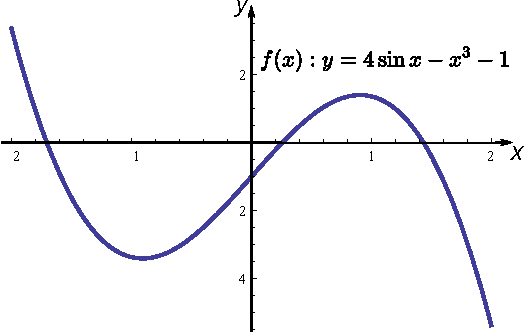
\includegraphics[scale=1]{mai_fig035.pdf}
           \captionof{figure}{Graf funkce $f(x):y=4\sin x - x^3 - 1$.}
           \label{mai:fig035}
           \par}
        Z obrázku \ref{mai:fig035} zjistíme, že existují tři kořeny: $x_1^*\in(-2,-1),
        x_2^*\in(-1, 0)$ a $x_3^*\in(1, 2)$.
      \end{example}
  
      Z obrázku zjistíme, že existují tři kořeny: $x_1^*\in(-2,-1),x_2^*\in(0,1),x_3^*\in(1,2)$.
      Zkusme najít kořeny v těchto intervalech pomocí numerických metod popsaných v následujících
      odstavcích
  
    \subsection{Metoda bisekce}
      Metoda známá také jako \textbf{metoda půlení intervalů}, je založena na principu
      zna\-mén\-ko\-vých změn. Předpokládejme, že funkce $f(x)$ má v koncových bodech intervalu
      $(a_0,b_0)$ opačná znaménka, tj. platí $f(a_0 )\cdot f(b_0 )<0$. Sestrojíme posloupnost
      intervalů $(a_1,b_1)\supset(a_2,b_2)\supset(a_3,b_3)\supset\cdots$, které obsahují kořen.
      Intervaly $(a_{k+1},b_{k+1}), k=0,1,\cdots$, určíme rekurzivně způsobem, který si nyní
      popíšeme.
  
      Střed intervalu $(a_k,b_k)$ je bod $x_{k+1}=\frac{1}{2}(a_k+b_k)$. Když $f(x_k)=0$, pak
      $x_{k+1}=x^*$ je kořen a dál nepokračujeme.

%} %tikzset
%---------------------------------------------------------------------------------------------------
%\printbibliography[heading=subbibliography]
\addcontentsline{toc}{section}{Seznam literatury}